\documentclass[11pt,a4paper,oneside]{report}
\usepackage{amsmath,amssymb,calc,ifthen}
\usepackage{float}
%\usepackage{cancel}
\usepackage[table,usenames,dvipsnames]{xcolor} % for coloured cells in tables
\usepackage{tikz}
% Allows us to click on links and references!
\usepackage{hyperref}
\usepackage{url}
\hypersetup{
colorlinks,
citecolor=black,
filecolor=black,
linkcolor=black,
urlcolor=black
}
% Nice package for plotting graphs
% See excellent guide:
% http://www.tug.org/TUGboat/tb31-1/tb97wright-pgfplots.pdf
\usetikzlibrary{plotmarks}
\usepackage{amsmath,graphicx}
\usepackage{epstopdf}
\usepackage{caption}
\usepackage{subcaption}
% highlight - useful for TODOs and similar
\usepackage{color}
\newcommand{\hilight}[1]{\colorbox{yellow}{#1}}
\newcommand\ci{\perp\!\!\!\perp} % perpendicular sign
\newcommand*\rfrac[2]{{}^{#1}\!/_{#2}} % diagonal fraction
\newcommand\SLASH{\char`\\}
\usepackage{listings}
% margin size
\usepackage[margin=1in]{geometry}
\tikzstyle{state}=[circle,thick,draw=black, align=center, minimum size=2.1cm,
inner sep=0]
\tikzstyle{vertex}=[circle,thick,draw=black]
\tikzstyle{terminal}=[rectangle,thick,draw=black]
\tikzstyle{edge} = [draw,thick]
\tikzstyle{lo} = [edge,dotted]
\tikzstyle{hi} = [edge]
\tikzstyle{trans} = [edge,->]
\definecolor{mygreen}{rgb}{0,0.6,0}
\definecolor{mygray}{rgb}{0.5,0.5,0.5}
\definecolor{mymauve}{rgb}{0.58,0,0.82}
\DeclareMathOperator*{\argmin}{arg\,min}
\DeclareMathOperator*{\argmax}{arg\,max}
\lstset{ %
backgroundcolor=\color{white}, % choose the background color; you must add
%\usepackage{color} or \usepackage{xcolor}
basicstyle=\footnotesize, % the size of the fonts that are used for the
%code
breakatwhitespace=false, % sets if automatic breaks should only happen
%at whitespace
breaklines=true, % sets automatic line breaking
captionpos=b, % sets the caption-position to bottom
commentstyle=\color{mygreen}, % comment style
deletekeywords={...}, % if you want to delete keywords from the
%given language
escapeinside={\%*}{*)}, % if you want to add LaTeX within your code
extendedchars=true, % lets you use non-ASCII characters; for
%8-bits encodings only, does not work with UTF-8
frame=single, % adds a frame around the code
keepspaces=true, % keeps spaces in text, useful for keeping
%indentation of code (possibly needs columns=flexible)
keywordstyle=\color{blue}, % keyword style
language=Octave, % the language of the code
morekeywords={*,...}, % if you want to add more keywords to the set
numbers=left, % where to put the line-numbers; possible
%values are (none, left, right)
numbersep=5pt, % how far the line-numbers are from the code
numberstyle=\tiny\color{mygray}, % the style that is used for the line-numbers
rulecolor=\color{black}, % if not set, the frame-color may be changed
%on line-breaks within not-black text (e.g. comments (green here))
showspaces=false, % show spaces everywhere adding particular
%underscores; it overrides 'showstringspaces'
showstringspaces=false, % underline spaces within strings only
showtabs=false, % show tabs within strings adding particular
%underscores
stepnumber=2, % the step between two line-numbers. If it's
%1, each line will be numbered
stringstyle=\color{mymauve}, % string literal style
tabsize=2, % sets default tabsize to 2 spaces
title=\lstname % show the filename of files included with
%\lstinputlisting; also try caption instead of title
}
\title{Graphical Models Coursework 2}
\author{
Razvan Valentin Marinescu\\
Student Number: 14060166\\
\texttt{razvan.marinescu.14@ucl.ac.uk}
\and
Konstantinos Georgiadis\\
Student Number: 14110861\\
\texttt{konstantinos.georgiadis.14@ucl.ac.uk}
}
\begin{document}
\belowdisplayskip=12pt plus 3pt minus 9pt
\belowdisplayshortskip=7pt plus 3pt minus 4pt
\maketitle{}

\section*{Exercise 1.20}

	We sent this one in an e-mail.

\section*{Exercise 5.7}

During the first stage we want to calculate:	

\begin{align*}
arg\max_{h_1,...,h_T}&\ p(h_1,...,h_T|x_1,...,x_T)=\\
arg\max_{h_1,...,h_T}&\ p(h_1,...,h_T,x_1,...,x_T)=\\
arg\max_{h_1,...,h_T}&\sum_{y_1,...,y_T}p(h_1,...,h_T,x_1,...,x_T,y_1,...,y_T)=\\		
arg\max_{h_1,...,h_T}&\sum_{y_1,...,y_T}p(x_1|h_1)p(y_1|h_1)p(h_1)\prod_{t=2}^Tp(h_t|h_{t-1})p(x_t|h_t)p(y_t|h_t)=\\	
arg\max_{h_1,...,h_T}&\ p(x_1|h_1)\left(\sum_{y_1}p(y_1|h_1)\right)p(h_1)\prod_{t=2}^Tp(h_t|h_{t-1})p(x_t|h_t)\left(\sum_{y_t}p(y_t|h_t)\right)=\\	
arg\max_{h_1,...,h_T}&\ p(x_1|h_1)p(h_1)\prod_{t=2}^Tp(h_t|h_{t-1})p(x_t|h_t)=\\		
arg\max_{h_1,...,h_T}&\ p(x_1|h_1)p(h_1)p(h_2|h_1)p(x_2|h_2)...p(h_T|h_{T-1})p(x_T|h_T)			
\end{align*}

By using the message passing and factor graph theory we can distribute the maximizations:

\begin{align*}
arg\max_{h_1,...,h_T}&\ p(x_1|h_1)p(h_1)p(h_2|h_1)p(x_2|h_2)...p(h_T|h_{T-1})p(x_T|h_T)=\\	
arg\max_{h_2,...,h_T}&\left(\max_{h_1} p(x_1|h_1)p(h_1)p(h_2|h_1)\right)p(x_2|h_2)...p(h_T|h_{T-1})p(x_T|h_T)=\\
arg\max_{h_2,...,h_T}&\ \mu_1(h_2)p(x_2|h_2)...p(h_T|h_{T-1})p(x_T|h_T)=\\
arg\max_{h_3,...,h_T}&\left(\max_{h_2}\ \mu_1(h_2)p(x_2|h_2)p(h_3|h_2)\right)...p(h_T|h_{T-1})p(x_T|h_T)=\\
arg\max_{h_3,...,h_T}&\ \mu_2(h_3)p(x_3|h_3)...p(h_T|h_{T-1})p(x_T|h_T)=...=arg\max_{h_T}\ \mu_{T-1}(h_T)p(x_T|h_T)
\end{align*}

Afterwards we need to perform the backtracking. In practice, in our code, every message $\mu_t(h_{t+1} = i)$ contains the probability $\max_{h_t}\ \mu_{t-1}(h_t)p(x_t|h_t)p(h_{t+1}=i|h_t)$, as well as the value for $h_t$ which gave that maximum probability, i.e. $arg\max_{h_t}\ \mu_{t-1}(h_t)p(x_t|h_t)p(h_{t+1}=i|h_t)$.

After we have found the optimal $h_1^\ast,...,h_T^\ast$, we want to compute:

\begin{align*}
arg\max_{y_1,...,y_T}&\ p(y_1,...,y_T|h_1^\ast,...,h_T^\ast)=\\
arg\max_{y_1,...,y_T}&\sum_{x_1,...,x_T}p(x_1|h_1^\ast)p(y_1|h_1^\ast)p(h_1^\ast)\prod_{t=2}^Tp(h_t^\ast|h_{t-1}^\ast)p(x_t|h_t^\ast)p(y_t|h_t^\ast)=\\
arg\max_{y_1,...,y_T}&\ p(y_1|h_1^\ast)p(h_1^\ast)\prod_{t=2}^Tp(h_t^\ast|h_{t-1}^\ast)p(y_t|h_t^\ast)
\end{align*}

However, we know the values of $h_1^\ast,...,h_T^\ast$, therefore we define:

$$K = p(h_1^\ast)\prod_{t=2}^Tp(h_t^\ast|h_{t-1}^\ast)$$

And so:

\begin{align*}
arg\max_{y_1,...,y_T}&\ p(y_1|h_1^\ast)p(h_1^\ast)\prod_{t=2}^Tp(h_t^\ast|h_{t-1}^\ast)p(y_t|h_t^\ast)=\\
arg\max_{y_1,...,y_T}&\ K\prod_{t=1}^Tp(y_t|h_t^\ast)=\\
arg&\ K\prod_{t=1}^T\max_{y_t}p(y_t|h_t^\ast)
\end{align*}

Which means that we can separately simply find each optimal $y_t^\ast$ for a given $h_t^\ast$ by maximizing $y_t^\ast=arg\max_{y_t}p(y_t|h_t^\ast)$ and not their product.\\

MATLAB code:
\begin{lstlisting}
clear all;clc;
load('banana.mat');
A = 1;
C = 2;
G = 3;
T = 4;

N = length(x);

%Convert DNA sequence x to X
X = cell(N,1);
for i = 1:1:N
    if(x(i) == 'A')
        X{i} = A;
    elseif(x(i) == 'C')
        X{i} = C;
    elseif(x(i) == 'G')
        X{i} = G;
    elseif(x(i) == 'T')
        X{i} = T;
    end
end

%Find optimal h given x
Messages = cell(N,1);
for j = 1:1:5
    [Messages{1}(j,1), Messages{1}(j,2)] = max(ph1.*pxgh(X{1},:)'.*phtghtm(j,:)');
end
for i = 2:1:N-1
    for j = 1:1:5
        [Messages{i}(j,1), Messages{i}(j,2)] = max(Messages{i-1}(:,1).*pxgh(X{i},:)'.*phtghtm(j,:)');
    end
end
[Messages{N}(1,1), Messages{N}(1,2)] = max(Messages{N-1}(:,1).*pxgh(X{N},:)');

%Backtracking to find optimal h
H = cell(N,1);
H{N} = Messages{N}(1,2);
for i = N-1:-1:1
    H{i} = Messages{i}(H{i+1},2);
end

%Finding optimal y given optimal h
Y = cell(N,1);
for i = 1:1:N
    [~,Y{i}] = max(pygh(:,H{i}));
end

%Convert Y to DNA sequence y
y = [];
for i = 1:1:N
    if(Y{i} == A)
        y = strcat(y,'A');
    elseif(Y{i} == C)
        y = strcat(y,'C');
    elseif(Y{i} == G)
        y = strcat(y,'G');
    elseif(Y{i} == T)
        y = strcat(y,'T');
    end
end

fprintf('Initial X sequence and Y sequence below:\n\n%s\n%s\n\n', x,y);
\end{lstlisting}

The output of the code is:\\\\
Initial X sequence and Y sequence below:\\\\
AAATCCAATCGAGCAACCCCATATGTGGAGTAGCGGACTAACTTCAACCG\\
ATGACAAAAAAAGTAATCAACTGACCGATCAACTATTCGATTCAGTAAAC\\\\
CTTGACTTGACTGACTGACTGACTGACCTGATTTTTTGACTGAGACTGAC\\
TGTTTTTTTTCTGACTGACTGACTGACTGACTGACTGACTGACTGACTGA\\\\

There is no computationally efficient way to compute:
$$arg\max_{y_1,...,y_T}\ p(y_1,...,y_T|x_1,...,x_T)$$
	If we try to use message passing theory, the messages will keep growing in size:

\begin{align*}
arg\max_{y_1,...,y_T}&\ p(y_1,...,y_T|x_1,...,x_T)=\\
arg\max_{y_1,...,y_T}&\sum_{h_1,...,h_T}p(x_1|h_1)p(y_1|h_1)p(h_1)\prod_{t=2}^Tp(h_t|h_{t-1})p(x_t|h_t)p(y_t|h_t)=\\
arg\max_{y_1,...,y_T}&\sum_{h_2,...,h_T}\left(\sum_{h_1}p(x_1|h_1)p(y_1|h_1)p(h_1)p(h_2|h_1)\right)p(x_2|h_2)p(y_2|h_2)\prod_{t=3}^Tp(h_t|h_{t-1})p(x_t|h_t)p(y_t|h_t)=\\
arg\max_{y_1,...,y_T}&\sum_{h_2,...,h_T}\mu_1(x_1,y_1,h_2)p(x_2|h_2)p(y_2|h_2)\prod_{t=3}^Tp(h_t|h_{t-1})p(x_t|h_t)p(y_t|h_t)=\\
arg\max_{y_1,...,y_T}&\sum_{h_3,...,h_T}\left(\sum_{h_2}\mu_1(x_1,y_1,h_2)p(x_2|h_2)p(y_2|h_2)p(h_3|h_2)\right)p(x_3|h_3)p(y_3|h_3)\prod_{t=4}^Tp(h_t|h_{t-1})p(x_t|h_t)p(y_t|h_t)=\\
arg\max_{y_1,...,y_T}&\sum_{h_3,...,h_T}\mu_2(x_1,y_1,x_2,y_2,h_3)p(x_3|h_3)p(y_3|h_3)\prod_{t=4}^Tp(h_t|h_{t-1})p(x_t|h_t)p(y_t|h_t)
\end{align*}

The messages $\mu_t(.)$ will keep growing and their size in memory (and therefore computations) are on the order of $O(5*4^{2t})$, which is exponential. Therefore, we cannot even calculate easily an instantiation of $p(y_1,...,y_T,x_1,...,x_T)$, let alone find its maximum.

\section*{Exercise 5.9}

	We attempted to do this exercise, but we could not figure out a way to find a precise solution to the problem, due to the very large number of variables and their domains. We first modeled the joint probability distribution. We decided that every person gets a variable describing their location at every timestep, i.e. $l_t^i$ is the variable for person i at timestep t, where $i \in \{1,...,500\}$ and $t \in \{1,...,100\}$. The domain of those variables are every pixel of the 50x50 board, i.e. $dom(l_t^i)=\{(1,1),(1,2),...,(1,50),(2,1),...,(50,50)\}$. The variable $l_t^1$ refers to the dangerous drunk. These are the hidden variables. We also assumed there are 100 observed variables - the board at every timestep - $O_t$. We modeled the joint distribution in the following way:
	
	$$p(\mathbf{l,O})=\left( \prod_{i=1}^{500}p(l_1^i) \right) \left( \prod_{i=1}^{500}p(l_2^i|l_1^i) \right) \left( \prod_{t=3}^{100} p(l_t^1|l_{t-1}^1) \left[ \prod_{i=2}^{500}p(l_t^i|l_{t-1}^i,l_{t-2}^i) \right] \right) \left( \prod_{t=1}^{100}p(O_t|l_t^1,...,l_t^{500}) \right)$$
	
	This joint distribution follows the code described in drunkmover.m. Specifically we defined every probability with the following code:

\begin{lstlisting}
pl_1 = zeros(50,50);
pl_1(3:1:47,3:1:47) = 1/((47-3+1)^2);

pl_2h1gl_1h1 = zeros(50,50,50,50);
for x = 3:1:47
    for y = 3:1:47
        pl_2h1gl_1h1(x+2,y+2,x,y) = 1;
    end
end

pl_2higl_1hi = zeros(50,50,50,50);
for x = 3:1:47
    for y = 3:1:47
        pl_2higl_1hi(x+1,y+1,x,y) = 1/4;
        pl_2higl_1hi(x-1,y+1,x,y) = 1/4;
        pl_2higl_1hi(x+1,y-1,x,y) = 1/4;
        pl_2higl_1hi(x-1,y-1,x,y) = 1/4;
    end
end

pl_th1gl_tm1h1 = zeros(50,50,50,50);
for x = 1:1:50
    for y = 1:1:50
        counter = 0;
        if(x + 2 > 50 || y + 2 > 50)
            counter = counter + 1;
        else
            pl_th1gl_tm1h1(x+2,y+2,x,y) = 1/4;
        end
        if(x + 2 > 50 || y - 2 < 1)
            counter = counter + 1;
        else
            pl_th1gl_tm1h1(x+2,y-2,x,y) = 1/4;
        end
        if(x - 2 < 1 || y + 2 > 50)
            counter = counter + 1;
        else
            pl_th1gl_tm1h1(x-2,y+2,x,y) = 1/4;
        end
        if(x - 2 < 50 || y - 2 < 1)
            counter = counter + 1;
        else
            pl_th1gl_tm1h1(x-2,y-2,x,y) = 1/4;
        end
        if(counter > 0)
            pl_th1gl_tm1h1(3:1:47,3:1:47,x,y) = pl_th1gl_tm1h1(3:1:47,3:1:47,x,y) + counter/(4*((47-3+1)^2));
        end
    end
end

pl_thigl_tm1hil_tm2hi = zeros(50,50,50,50,50,50);
for x1 = 1:1:50
    for y1 = 1:1:50
        for x2 = 1:1:50
            for y2 = 1:1:50
                probsumto = 0;
                if(x1 + sign(x1-x2) > 50 || x1 + sign(x1-x2) < 1 || y1 + sign(y1-y2) > 50 || y1 + sign(y1-y2) < 1)
                    probsumto = probsumto + 0.99*0.99;
                else
                    pl_thigl_tm1hil_tm2hi(x1+sign(x1-x2),y1+sign(y1-y2),x1,y1,x2,y2) = 0.99*0.99;
                end
                if(x1 - sign(x1-x2) > 50 || x1 - sign(x1-x2) < 1 || y1 + sign(y1-y2) > 50 || y1 + sign(y1-y2) < 1)
                    probsumto = probsumto + 0.99*0.01;
                else
                    pl_thigl_tm1hil_tm2hi(x1-sign(x1-x2),y1+sign(y1-y2),x1,y1,x2,y2) = 0.99*0.01;
                end
                if(x1 + sign(x1-x2) > 50 || x1 + sign(x1-x2) < 1 || y1 - sign(y1-y2) > 50 || y1 - sign(y1-y2) < 1)
                    probsumto = probsumto + 0.99*0.01;
                else
                    pl_thigl_tm1hil_tm2hi(x1+sign(x1-x2),y1-sign(y1-y2),x1,y1,x2,y2) = 0.99*0.01;
                end
                if(x1 - sign(x1-x2) > 50 || x1 - sign(x1-x2) < 1 || y1 - sign(y1-y2) > 50 || y1 - sign(y1-y2) < 1)
                    probsumto = probsumto + 0.01*0.01;
                else
                    pl_thigl_tm1hil_tm2hi(x1-sign(x1-x2),y1-sign(y1-y2),x1,y1,x2,y2) = 0.01*0.01;
                end
                if(probsumto > 0)
                    pl_thigl_tm1hil_tm2hi(3:1:47,3:1:47,x1,y1,x2,y2) = pl_thigl_tm1hil_tm2hi(3:1:47,3:1:47,x1,y1,x2,y2) + (1-probsumto)*(1/(47-3+1)^2);
                end
            end
        end
    end
end
\end{lstlisting}

where:\\
\begin{align*}
p(l_1^i=(x,y))&\ is\ pl\_1(x,y)\\
p(l_2^1=(x,y)|l_1^1=(x',y'))&\ is\ pl\_2h1gl\_1h1(x,y,x',y')\\
p(l_2^i=(x,y)|l_1^i=(x',y'))&\ is\ pl\_2higl\_1hi(x,y,x',y')\\
p(l_t^1=(x,y)|l_{t-1}^1=(x',y'))&\ is\ pl\_th1gl\_tm1h1(x,y,x',y')\\
p(l_t^i=(x,y)|l_{t-1}^i=(x_{-1},y_{-1}),l_{t-2}^i=(x_{-2},y_{-2}))&\ is\ pl\_thigl\_tm1hil\_tm2hi(x,y,x_{-1},y_{-1},x_{-2},y_{-2})
\end{align*}

Regarding the observed variables $p(O_t|l_t^1,...,l_t^{500})=1$ when all the variables $l_t$ are in the positions that are occupied in the grid and also that for every occupied location in the grid, there is at least one $l_t$ variable with the x,y coordinates that describe the location. We are now posed with the following two optimization problems:
\begin{align*}
&arg\max_{l_T^1}p(l_T^1 | O_1,...,O_T)\\
&arg\max_{l_1^1,...,l_{100}^1}p(l_1^1,...,l_{100}^1 | O_1,...,O_{100})\\
\end{align*}
Herein lies our problem, as we need to sum over all $l_t^i$ variables $\forall i \neq 1$. This means that at some point we will need to calculate $p(O_t|l_t^1,...,l_t^{500})$. Even with this problem alone, we can simplify it, by only taking into account all the possible permutations (or even just combinations) of $l_t^i$s that make this probability equal to one, but even in that case, there are still a lot of permutations or combinations of these variables that satisfy this. In any case, we were not able to think of an exact solution for these problems. 

\section*{Exercise 5.11}	

Calculating recursively the positions at every timestep:
\begin{align*}
x_2 &= x_1 + \delta v_1\\
x_3 &= x_2 + \delta v_2 = x_1 + \delta v_1 + \delta v_2 = x_1 + \delta (v_1+v_2)\\
\text{We can therefore derive that:}&\\
x_t &= x_1 + \delta \sum_{i=1}^{t-1}v_i\\
x_{102} &= x_1 + \delta \sum_{i=1}^{101}v_i\\
\text{We also have:}&\\
v_2 &= v_1 + \delta a_1\\
v_3 &= v_2 + \delta a_2 = v_1 + \delta (a_1+a_2)\\
v_t &= v_1 + \delta \sum_{i=1}^{t-1}a_i\\
x_{102} &= x_1 + \delta \sum_{i=1}^{101} v_1 + \delta \sum_{j=1}^{i-1}a_j\\
\text{But we know that:}\ & x_1 = [ 0\ 0\ 0 ]^\top, v_1 = [0\ 0\ 0]^\top \ \text{therefore:} \\
x_{102} &= \delta^2 \sum_{i=1}^{101}\sum_{j=1}^{i-1}a_j\\
x_{102} &= \delta^2 \sum_{i=2}^{101}\sum_{j=1}^{i-1}a_j\\
x_{102} &= \delta^2 (100a_1+99a_2+...+2a_{99}+a_{100})\\
\text{Therefore we have that:}&\\
4.71 &= 0.01(100a_1(1)+99a_1(2)+...+2a_1(99)+a_1(100))\\
-6.97 &= 0.01(100a_2(1)+99a_2(2)+...+2a_2(99)+a_2(100))\\
8.59 &= 0.01(100a_3(1)+99a_3(2)+...+2a_3(99)+a_3(100))\\
471 &= 100a_1(1)+99a_1(2)+...+2a_1(99)+a_1(100)\\
-697 &= 100a_2(1)+99a_2(2)+...+2a_2(99)+a_2(100)\\
859 &= 100a_3(1)+99a_3(2)+...+2a_3(99)+a_3(100)\\
\end{align*}

In order to calculate the minimum fuel used, we look at each dimension separately. Basically, we have all the integer numbers between 1 and 100 and we can choose which ones to add up(or subtract), but they need to add up to 471, -697, 859 in each dimension respectively. Thus, it makes sense to do the following. At every iteration, we choose the number available which gets us as close as possible to the one desired. For example with the first dimension, we want to reach 471 at timestep 102, therefore we choose:\\
100,99,98,97 and 77, which added up equals 471. This means that $a_1(1)=1, a_1(2)=1, a_1(3)=1,a_1(4)=1,a_1(24)=1$ and $a_1(t) = 0,\ \forall t \in \{5,...,23,25,...,100\}$
More specifically, we first choose $a_1(1) = 1$, because if we subtract that number from 471, it is the one that gets us closest to zero, i.e. $471-100a_1(1) = 471-100=371$. Afterwards we repeat the same for $a_1(2)=1, a_1(3)=1,a_1(4)=1$ and we are left with $471-100a_1(1)-99a_1(2)-98a_1(3)-97a_1(4)=77$ and so we choose $a_1(24)=1$. This is of course, not the only solution to the problem, as we can choose any combination that adds up to 471. For example we could also have chosen the numbers 100,99,98,96,78. However, in order to be sure that we used the minimum fuel needed, our approach will always work.\\
Likewise for the second dimension we have:\\
$a_2(1)=-1,a_2(2)=-1,a_2(3)=-1,a_2(4)=-1,a_2(5)=-1,a_2(6)=-1,a_2(7)=-1,a_2(83)=-1$ and $a_2(t)=0,\ \forall t\in \{8,...,82,84,...,100\}$\\
And for the third dimension we have:\\
$a_3(1)=1,a_3(2)=1,a_3(3)=1,a_3(4)=1,a_3(5)=1,a_3(6)=1,a_3(7)=1,a_3(8)=1,a_3(14)=1$ and $a_3(t)=0,\ \forall t\in \{9,...,13,15,...,100\}$\\

Therefore the total minimum amount of fuel needed is $5+8+9=22$.\\

If we also want at the same time to have 0 speed at timestep 102, then we now have two conditions that need to be met (we assumed that we can also accelerate at timestep 101, otherwise we need have reached the coordinated at timestep 101 already and not move at all at timestep 102. Our assumption does not make a huge difference for the solution either way):

\begin{align*}
0 &= a_1(1)+a_1(2)+...+a_1(99)+a_1(100)+a_1(101)\\
0 &= a_2(1)+a_2(2)+...+a_2(99)+a_2(100)+a_2(101)\\
0 &= a_3(1)+a_3(2)+...+a_3(99)+a_3(100)+a_3(101)\\
471 &= 100a_1(1)+99a_1(2)+...+2a_1(99)+a_1(100)\\
-697 &= 100a_2(1)+99a_2(2)+...+2a_2(99)+a_2(100)\\
859 &= 100a_3(1)+99a_3(2)+...+2a_3(99)+a_3(100)\\
\end{align*}

The new restrictions basically tell us that we need to have equal number of +1s and -1s. Still, our approach to solving this problem remains similar. Now we will choose couples of numbers, where the one will be a +1 and the other -1 and their sum will get us as close to zero as possible. For example, with the first dimension we first choose $a_1(1) = 1, a_1(101) = -1$. We can now subtract 100 from 471 and are left with 371. Next, we choose $a_1(2) = 1, a_1(100) = -1$. These two add up to $99-1=98$. Subtracting this from 371, we get 273. With the same principle we then choose $a_1(3)=1,a_1(99)=-1$ and $a_1(4)=1,a_1(98)=-1$. After subtracting those numbers as well, we are left with 83. Now we have a choice, since $a_1(5)=1,a_1(97)=-1$ would give us 92, which is more than 83. We can now adjust one or the other (or both), so that their sum will equal 83 exactly. We chose the couple $a_1(5)=1,a_1(88)=-1$ and $a_1(t)=0,\ \forall t \in \{6,...,87,89,...,97\}$. Therefore we have:\\
$471 = 100 + 99 + 98 + 97 + 96 - 0 - 1 - 2 - 3 - 13$\\
Likewise for the second dimension we have:\\
$a_2(1)=-1,a_2(101)=1,\ a_2(2)=-1,a_2(100)=1,\ a_2(3)=-1,a_2(99)=1,\ a_2(4)=-1,a_2(98)=1,\ a_2(5)=-1,a_2(97)=1,\ a_2(6)=-1,a_2(96)=1,\ a_2(7)=-1,a_2(95)=1,\ a_2(8)=-1,a_2(55)=1$ and $a_2(t)=0,\ \forall t \in \{9,...,54,56,...,94\}$\\
And for the third dimension we have:\\
$a_3(1)=1,a_3(101)=-1,\ a_3(2)=1,a_3(100)=-1,\ a_3(3)=1,a_3(99)=-1,\ a_3(4)=1,a_3(98)=-1,\ a_3(5)=1,a_3(97)=-1,\ a_3(6)=1,a_3(96)=-1,\ a_3(7)=1,a_3(95)=-1,\ a_3(8)=1,a_3(94)=-1,\ a_3(9)=1,a_3(93)=-1,\ a_3(10)=1,a_3(41)=-1,\ $ and $a_2(t)=0,\ \forall t \in \{11,...,40,42,...,92\}$\\

Therefore the total minimum amount of fuel needed is $10+16+20=46$

\section*{Exercise 5.13}

We wrote the following code for this exercise. It simply changes the matrix A to have the "edge weights" in the proper format for the mostprobablepath function.

\begin{lstlisting}
clear all; clc;
import brml.*
load('SimoHurrta.mat');
for i = 1:1:2000
    for j = 1:1:2000
        if(A(i,j) == 1)
            %replace value with the edge weight
            A(i,j) = -(norm(x(:,i)-x(:,j))-t(j));
        else
            A(i,j) = -inf;
        end
    end
end
[optpath, pathweight]=mostprobablepath(A',1,1725);
fprintf('The minimum cost of travelling from planet 1 to 1725 is: %f\n',-pathweight); 
\end{lstlisting}

The MATLAB outputs:

The minimum cost of travelling from planet 1 to 1725 is: -209.649903

\section*{Exercise 6.2}
	
	The clique graph:
	\begin{center} 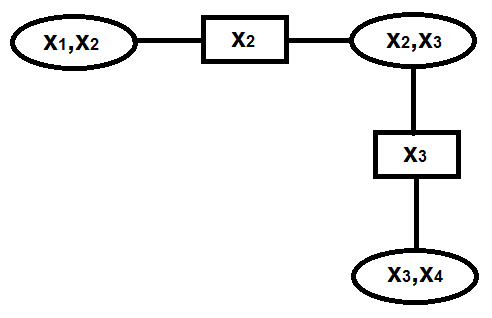
\includegraphics[width=0.75\textwidth]{c6e2clique}\end{center}  
	The separators are the variables in square boxes ($x_2$ and $x_3$).
	
\begin{align*}
p(x_1,x_2,x_3,x_4) &= \frac{\phi(x_1,x_2)\phi(x_2,x_3)\phi(x_3,x_4)}{Z}\\
Zp(x_1,x_2) &=\phi(x_1,x_2)\sum_{x_3,x_4}\phi(x_2,x_3)\phi(x_3,x_4)\\
Zp(x_2,x_3) &=\phi(x_2,x_3)\sum_{x_1}\phi(x_1,x_2)\sum_{x_4}\phi(x_3,x_4)\\
Zp(x_3,x_4) &=\phi(x_3,x_4)\sum_{x_1,x_2}\phi(x_1,x_2)\phi(x_2,x_3)\\
Therefore:&\\
Z^3p(x_1,x_2)p(x_2,x_3)p(x_3,x_4) &=\\ 
\phi(x_1,x_2)\phi(x_2,x_3)\phi(x_3,x_4)&\sum_{x_1,x_3,x_4}\phi(x_1,x_2)\phi(x_2,x_3)\phi(x_3,x_4)\sum_{x_1,x_2,x_4}\phi(x_1,x_2)\phi(x_2,x_3)\phi(x_3,x_4)\\
Z^3p(x_1,x_2)p(x_2,x_3)p(x_3,x_4) &= Zp(x_1,x_2,x_3,x_4)\sum_{x_1,x_3,x_4}Zp(x_1,x_2,x_3,x_4)\sum_{x_1,x_2,x_4}Zp(x_1,x_2,x_3,x_4)\\
Z^3p(x_1,x_2)p(x_2,x_3)p(x_3,x_4) &= Z^3p(x_1,x_2,x_3,x_4)p(x_2)p(x_3)\\
p(x_1,x_2,x_3,x_4) &= \frac{p(x_1,x_2)p(x_2,x_3)p(x_3,x_4)}{p(x_2)p(x_3)}\\
\end{align*}

\section*{Exercise 6.3}

After triangulating the markov network graph, we can get the following clique graph/junction tree:
	\begin{center} 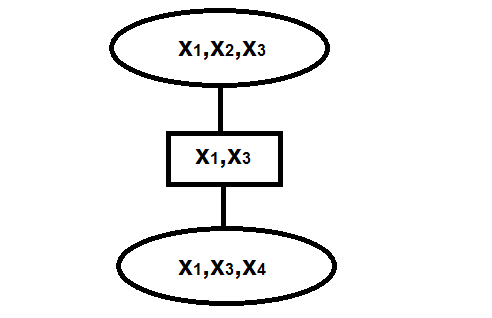
\includegraphics[width=0.75\textwidth]{c6e3junction}\end{center}  

We make the following assignments:
\begin{align*}
\phi(x_1,x_2,x_3) &= \phi(x_1,x_2)\phi(x_2,x_3)\\
\phi(x_1,x_3) &= 1\\
\phi(x_1,x_3,x_4) &= \phi(x_3,x_4)\phi(x_4,x_1)
\end{align*}

First, we perform the absorption $\phi(x_1,x_2,x_3)\rightarrowtail\phi(x_1,x_3,x_4)$:
\begin{align*}
\phi^\ast(x_1,x_3) &=\sum_{x_2}\phi(x_1,x_2,x_3)=\sum_{x_2}\phi(x_1,x_2)\phi(x_2,x_3) \\
\phi^\ast(x_1,x_3,x_4) &= \phi(x_1,x_3,x_4)\frac{\phi^\ast(x_1,x_3)}{\phi(x_1,x_3)}=\phi(x_3,x_4)\phi(x_4,x_1)\sum_{x_2}\phi(x_1,x_2)\phi(x_2,x_3)=p(x_1,x_3,x_4)
\end{align*}
We could perform the marginalization to calculate $p(x_1)$ right now, but we continued the absorption with $\phi^\ast(x_1,x_3,x_4)\rightarrowtail\phi(x_1,x_2,x_3)$:
\begin{align*}
\phi^{\ast\ast}(x_1,x_3) &=\sum_{x_4}\phi^\ast(x_1,x_3,x_4)=p(x_1,x_3) \\
\phi^\ast(x_1,x_2,x_3) &= \phi(x_1,x_2,x_3)\frac{\phi^{\ast\ast}(x_1,x_3)}{\phi^\ast(x_1,x_3)}=\frac{\phi(x_1,x_2)\phi(x_2,x_3)p(x_1,x_3)}{\sum_{x_2}\phi(x_1,x_2)\phi(x_2,x_3)}=\\
&=\frac{\phi(x_1,x_2)\phi(x_2,x_3)\sum_{x_2,x_4}\phi(x_1,x_2)\phi(x_2,x_3)\phi(x_3,x_4)\phi(x_4,x_1)}{\sum_{x_2}\phi(x_1,x_2)\phi(x_2,x_3)}=\\
&=\phi(x_1,x_2)\phi(x_2,x_3)\sum_{x_4}\phi(x_3,x_4)\phi(x_4,x_1)=p(x_1,x_2,x_3)
\end{align*}

Here is the code we used to verify the absorption and marginal calculation:
\begin{lstlisting}
clear all; clc;
import brml.*

%random potentials
Phix1x2 = [5 6; 1 3];
Phix2x3 = [4 9; 9 1];
Phix3x4 = [8 2; 5 12];
Phix4x1 = [12 6; 1 2];

x1 = 1;
x2 = 2;
x3 = 3;
x4 = 4;

fl=1; tr=2;
variable(x1).domain={'0','1'};
variable(x2).domain={'0','1'};
variable(x3).domain={'0','1'};
variable(x4).domain={'0','1'};
variable(1).name='X1';
variable(2).name='X2';
variable(3).name='X3';
variable(4).name='X4';

temppot = array([x1,x2]);
temppot.table = Phix1x2;
pot{1} = temppot;

temppot = array([x2,x3]);
temppot.table = Phix2x3;
pot{2} = temppot;

temppot = array([x3,x4]);
temppot.table = Phix3x4;
pot{3} = temppot;

temppot = array([x4,x1]);
temppot.table = Phix4x1;
pot{4} = temppot;

%Normal calculation
jointpot = multpots(pot([1:4])); 
Z = sum(sum(sum(sum(jointpot.table))));
jointpot.table = jointpot.table / Z;

marginalpot{1} = sumpot(jointpot,1,0);

%Calculation through junction tree absorption
junctionpot{1} = multpots(pot([1 2]));
junctionpot{2} = array([x1,x3]);
junctionpot{3} = multpots(pot([3 4]));
junctionpot{1}.table = junctionpot{1}.table/Z;

[junctionpotstar{2},junctionpotstar{3}] = absorb(junctionpot{1},junctionpot{2},junctionpot{3},[1 3]);
absorbmarginalpot{1} = sumpot(junctionpotstar{3},1,0);

%Comparison of results
[marginalpot{1}.table(tr) absorbmarginalpot{1}.table(tr)
marginalpot{1}.table(fl) absorbmarginalpot{1}.table(fl)]
\end{lstlisting}

At the end MATLAB outputs(format longg):\\

ans =\\
         0.171419902912621         0.171419902912621\\
         0.828580097087379         0.828580097087379\\
         
Since the elements of the rows are the same, the calculation was done correctly.

\section*{Exercise 6.7}

We describe below our reasoning with a 3x3 lattice and then find the computational cost for the general case:

	\begin{center} 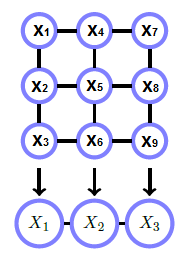
\includegraphics[width=0.25\textwidth]{c6e7temp}\end{center}  
	
	In this case $X_1$ consists of $x_1,x_2,x_3$. Likewise, $X_2$ consists of $x_4,x_5,x_6$ and similarly for $X_3$. The junction tree is:
	
	\begin{center} 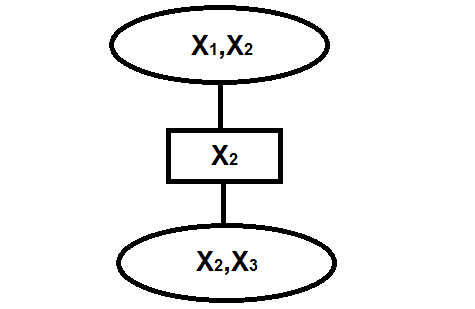
\includegraphics[width=0.5\textwidth]{c6e7clique}\end{center}  

Where $\phi(X_1,X_2) = \phi(x_1,x_2,x_3,x_4,x_5,x_6)$ and $\phi(X_2,X_3) = \phi(x_4,x_5,x_6,x_7,x_8,x_9)$. We can now assign each potential to a clique of the junction tree. We chose the following assignment:
\begin{align*}
\phi(X_1,X_2) &= \phi(x_1,x_2)\phi(x_2,x_3)\phi(x_1,x_4)\phi(x_2,x_5)\phi(x_3,x_6)\phi(x_4,x_5)\phi(x_5,x_6)\\
\phi(X_2) &= 1\\
\phi(X_2,X_3) &= \phi(x_7,x_8)\phi(x_8,x_9)\phi(x_4,x_7)\phi(x_5,x_8)\phi(x_6,x_9)
\end{align*}
The idea is then to perform absorptions from one end to the other and then we can calculate $Z$ by summing over the variables of the last clique and its updated potential, as shown in the theory in the book. In this case the steps for the absorption are:
\begin{align*}
\phi^\ast(X_2) &= \sum_{X_1}\phi(X_1,X_2) = \sum_{x_1,x_2,x_3}\phi(x_1,x_2)\phi(x_2,x_3)\phi(x_1,x_4)\phi(x_2,x_5)\phi(x_3,x_6)\phi(x_4,x_5)\\
\phi^\ast(X_2,X_3) &= \phi(X_2,X_3)\frac{\phi^\ast(X_2)}{\phi(X_2)}=\phi(X_2,X_3)\phi^\ast(X_2)
\end{align*}

We will now describe the absorption steps in the NxN lattice case, which utilizes the fact that separators are initialized to the value 1:
\begin{align*}
\phi^\ast(X_2) &= \sum_{X_1}\phi(X_1,X_2)\\
\phi^\ast(X_2,X_3) &= \phi(X_2,X_3)\frac{\phi^\ast(X_2)}{\phi(X_2)}=\phi(X_2,X_3)\sum_{X_1}\phi(X_1,X_2)\\
\phi^\ast(X_3) &= \sum_{X_2}\phi^\ast(X_2,X_3)\\
\phi^\ast(X_3,X_4) &= \phi(X_3,X_4)\frac{\phi^\ast(X_3)}{\phi(X_3)}=\phi(X_3,X_4)\sum_{X_2}\phi^\ast(X_2,X_3)=\phi(X_3,X_4)\sum_{X_2}\phi(X_2,X_3)\sum_{X_1}\phi(X_1,X_2)\\
&...\\
\phi^\ast(X_{N-1},X_N)&=\phi(X_{N-1},X_N)\sum_{X_{N-2}}\phi(X_{N-2},X_{N-1})...\sum_{X_1}\phi(X_1,X_2)
\end{align*}
And since we want to calculate $Z$, we want:
\begin{align*}
Z=\sum_{X_{N-1},X_N}\phi^\ast(X_{N-1},X_N)=\sum_{X_{N-1},X_N}\phi(X_{N-1},X_N)\sum_{X_{N-2}}\phi(X_{N-2},X_{N-1})...\sum_{X_1}\phi(X_1,X_2)
\end{align*}
Therefore the required calculations are:\\
1. We first need to calculate every $\phi(X_i,X_{i+1})$. Each $X_i$ variable will now take $2^N$ states, therefore every $\phi(X_i,X_{i+1})$ requires calculation for $2^{2N}$ states. Each calculation for a specific state $\phi(X_i = a,X_{i+1} = b)$ requires the multiplication of $(N-1)+N+(N-1)$ numbers for $\phi(X_1,X_2)$ and $(N-1)+N$ for all other $\phi(X_i,X_{i+1})$. Therefore, we require $3(N-1)$ and $2(N-1)$ multiplications respectively. Due to the specific nature of the potentials in this case, we could also just check how many edges connect $x_i$ variables with in the same state. If we assume there are $K$ such edges, then the potential is $e^K$. In any case, the complexity does not really change. We also have $N-1$ such $\phi(X_i,X_{i+1})$, however the matrices representing them will all be the same for $i>1$, therefore the total complexity to initialize the new markov network is $2^{2N}(2(N-1)+3(N-1))=2^{2N}5(N-1)$\\
2. We now want to do the message passing. For $\sum_{X_1}\phi(X_1,X_2)$ we are going to end up with a new function $\mu(X_2)$ with $2^N$ states and each state requiring the summation of $2^N$ numbers, therefore $2^N(2^N-1)$ additions. For all other summations over some variable except the last one we now have $\sum_{X_i}\phi(X_i,X_{i+1})\mu(X_i)$. Now, the messages $\mu(X_{i+1})$ with $2^N$ will require $2^N$ multiplications and $2^N-1$ additions for every state, therefore a total of $2^N(2^{N+1}-1)$ computations. There will be $N-3$ such messages. Lastly, we need to calculate $\sum_{X_{N-1},X_N}\phi(X_{N-1},X_N)\mu(X_{N-1})$ which requires $2^{2N}$ multiplications and $2^{2N}-1$ additions. Therefore the total computational cost is $2^N(2^N-1)+(N-3)2^N(2^{N+1}-1)+2^{2N}+2^{2N}-1=(N-2)(2^{2N+1}-2^N)+2^{2N}-1$.\\

For $N=10$, the computational cost is 47185920 calculations for the initialization and 17817599 calculations to calculate Z. MATLAB code to calculate the logarithm of Z for N = 10:\\

\begin{lstlisting}
clear all; clc;
import brml.*

N = 10;
Phixixj = [exp(1) exp(0); exp(0) exp(1)];

fl=1; tr=2;

temppot = array([1,2]);
for i = 0:1:2^N-1
    for j = 0:1:2^N-1
        %convert to binary states
        X_i = zeros(1,10);
        temp = de2bi(i);
        X_i(1:length(temp)) = temp;
        X_j = zeros(1,10);
        temp = de2bi(j);
        X_j(1:length(temp)) = temp;
        %count number of edges with their nodes being in the same state
        temppot.table(i+1,j+1) = exp(sum(X_i == X_j) + sum(X_i(1:end-1)==X_i(2:end)) + sum(X_j(1:end-1)==X_j(2:end)));
    end
end
pot{1} = temppot;

temptable = zeros(2^N);
for i = 0:1:2^N-1
    for j = 0:1:2^N-1
        %convert to binary states
        X_i = zeros(1,10);
        temp = de2bi(i);
        X_i(1:length(temp)) = temp;
        X_j = zeros(1,10);
        temp = de2bi(j);
        X_j(1:length(temp)) = temp;
        temptable(i+1,j+1) = exp(sum(X_i == X_j) + sum(X_j(1:end-1)==X_j(2:end)));
    end
end


for l = 2:1:9
    temppot = array([l,l+1]);
    temppot.table = temptable;
    pot{l} = temppot;
end

separator = array();

%Absorption Procedure
potstar{1} = pot{1};
for l = 2:1:9
[temp,potstar{l}] = absorb(potstar{l-1},separator,pot{l},l);
end

logZ = log(sum(sum(potstar{9}.table)));
fprintf('The logarithm of Z is: %f\n', logZ);
\end{lstlisting}

MATLAB outputs:\\\\

The logarithm of Z is: 186.791621

\section*{Exercise 6.9}

We used the following code for the three questions. For the first question, after doing a full absorption, we simply find a clique which contains the variable we want to find the marginal for and calculate it. For the second question, we notice that we can do the following calculation instead:
\begin{align*}
p(s_i) &= \sum_{s \SLASH s_i,d_1,...,d_{20}}p(s_1,...,s_40,d_1,...,d_20)\\
&= \sum_{s \SLASH s_i,d_1,...,d_{20}} \prod_{j=1}^{20} p(d_j) p(s_1|d_a,d_b,d_c)...p(s_40|d_d,d_e,d_f)\\
&= \sum_{d_1,...,d_{20}} \prod_{j=1}^{20} p(d_j) p(s_i|d_a,d_b,d_c)\\
&= \sum_{d_a,d_b,d_c} p(s_i|d_a,d_b,d_c)p(d_a)p(d_b)p(d_c)\\
\end{align*}

And our MATLAB code outputs the maximum difference between the two methods of calculating the marginals:\\

Maximum Error: 2.731149e-14\\

Lastly, we set the states of $s_1,...,s_{10}$ to their evidence states, then rerun the JTA algorithm and calculate the marginal for every disease. We compare the marginals of the diseases in state 1 without the evidence (1st row) to the marginals of the diseases in state 1 with the evidence (2nd row) in the variable ProbabilityChange. \\

ProbabilityChange =\\
  Columns 1 through 3\\
        0.0297756150056143         0.703369715389595         0.890035806411971\\
        0.0297756150056363         0.381760210392638         0.954234885012652\\
  Columns 4 through 6\\
         0.356960781594245         0.441540870657941         0.440297774283691\\
         0.396644439744307         0.496467474143678         0.435154394247795\\
  Columns 7 through 9\\
         0.537922483558776         0.645047642235049        0.0471565296117175\\
         0.187487234010803         0.701182817776376        0.0431266480981353\\
  Columns 10 through 12\\
          0.56423881513303         0.360280208988753         0.516823199366758\\
         0.610312518956601         0.287322294475541         0.489833195166836\\
  Columns 13 through 15\\
         0.893383217820786         0.659791679227307          0.92047572757886\\
         0.899599829793571         0.619564596616766         0.920475727580807\\
  Columns 16 through 18\\
         0.457154265322789         0.168814086782772         0.896173814389867\\
         0.706096164794708         0.201247206425337         0.908494315475222\\
  Columns 19 through 20\\
         0.735003557843084         0.761318781486525\\
         0.864967251455448         0.883929046039115\\
         
	We can see that for disease 1 and 15 there was no change, which is to be expected, since none of the symptoms with evidence depended on them. All of the other marginals have changed as they should have.         

\begin{lstlisting}
clear all; clc;
import brml.*
load('diseaseNet.mat');
[jtpot, jtsep, infostruct]=jtree(pot);
[jtpotfullabsorb, jtsepfullabsorb, Z]=absorption(jtpot,jtsep,infostruct); % do full round of absorption

%Calculate Symptom marginals with the JT algorithm
CalculatedMarginals = false(1,40);
while(1)
    for i = 1:1:length(jtpotfullabsorb)
        for j = jtpotfullabsorb{i}.variables
            if(j > 20)
                if(~CalculatedMarginals(j-20))
                    SymptomMarginalsJT{j-20} = sumpot(jtpotfullabsorb{i},j,0);
                    CalculatedMarginals(j-20) = true;
                    if(sum(CalculatedMarginals) == 40)
                        break;
                    end
                end
            end
        end
        if(sum(CalculatedMarginals) == 40)
            break;
        end
    end
    if(sum(CalculatedMarginals) == 40)
        break;
    end
end

%Compute Symptom marginals with simple Belief Network Inference
for i = 1:1:40
    SymptomMarginalsBN{i} = sumpot(multpots(pot(pot{i+20}.variables)),i+20,0);
end

%Compute Error between the two methods
for i = 1:1:40
    MarginalErrors(:,i) = abs(SymptomMarginalsBN{i}.table-SymptomMarginalsJT{i}.table);
end
fprintf('Maximum Error: %e\n', max(max(MarginalErrors)));

%3rd part of exercise. Setting variables with evidence to their evidence
%state
for i = 1:1:60
    potcond{i} = setpot(pot{i},[21:1:30], [1 1 1 1 1 2 2 2 2 2]);
end
[newpot, newvars, uniquevariables, uniquenstates] = squeezepots(potcond);

[jtpotcond, jtsepcond, infostructcond]=jtree(newpot);
[jtpotfullabsorbcond, jtsepfullabsorbcond, Zcond]=absorption(jtpotcond,jtsepcond,infostructcond); % do full round of absorption
for i = 1:1:length(jtpotfullabsorbcond)
    jtpotfullabsorbcond{i}.table = jtpotfullabsorbcond{i}.table/Zcond;
end

%Calculate Disease marginals with the JT algorithm with the conditions
CalculatedMarginals = false(1,20);
while(1)
    for i = 1:1:length(jtpotfullabsorbcond)
        for j = jtpotfullabsorbcond{i}.variables
            if(j < 21)
                if(~CalculatedMarginals(j))
                    DiseaseMarginalsJT{j} = sumpot(jtpotfullabsorbcond{i},j,0);
                    CalculatedMarginals(j) = true;
                    if(sum(CalculatedMarginals) == 20)
                        break;
                    end
                end
            end
        end
        if(sum(CalculatedMarginals) == 20)
            break;
        end
    end
    if(sum(CalculatedMarginals) == 20)
        break;
    end
end

%Calculate Disease marginals with the JT algorithm without the conditions
CalculatedMarginals = false(1,20);
while(1)
    for i = 1:1:length(jtpotfullabsorb)
        for j = jtpotfullabsorb{i}.variables
            if(j < 21)
                if(~CalculatedMarginals(j))
                    DiseaseMarginalsJTuncond{j} = sumpot(jtpotfullabsorb{i},j,0);
                    CalculatedMarginals(j) = true;
                    if(sum(CalculatedMarginals) == 20)
                        break;
                    end
                end
            end
        end
        if(sum(CalculatedMarginals) == 20)
            break;
        end
    end
    if(sum(CalculatedMarginals) == 20)
        break;
    end
end

%Check if there has been a difference in the marginals with the conditions
for i = 1:1:20
    ProbabilityChange(:,i) = [DiseaseMarginalsJTuncond{i}.table(1);DiseaseMarginalsJT{i}.table(1)];
end
\end{lstlisting}

\section*{Exercise 6.10}

Due to the moralization step when trying to create a junction tree for this probability distribution, every variable will be connected to every variable. This means there will only be one clique which will include all the variables: $\phi(x_1,...,x_T,y) = p(x_1)\prod_{i=2}^Tp(x_i|x_{i-1})p(y|x_1,...,x_T)$. In order to then calculate $p(x_T)$ we need to sum over all other variables. This means that for each of the two states of $x_T$ we need the sum of $2^T$ numbers (since the total variables are $T+1$), therefore the total computational cost is $2(2^T-1)$ additions.

By simply using message passing theory from the previous chapter we can:
\begin{align*}
p(x_T)&=\sum_{x_1,...,x_{T-1},y}p(x_1)\prod_{i=2}^Tp(x_i|x_{i-1})p(y|x_1,...,x_T)=\\
&=\sum_{x_1,...,x_{T-1}}p(x_1)\prod_{i=2}^Tp(x_i|x_{i-1})=\\
&=\sum_{x_2,...,x_{T-1}}\left(\sum_{x_1}p(x_1)p(x_2|x_1)\right)\prod_{i=3}^Tp(x_i|x_{i-1})=\\
&=\sum_{x_2,...,x_{T-1}}\mu(x_2)\prod_{i=3}^Tp(x_i|x_{i-1})=\\
&...\\
&=\sum_{x_{T-1}}\mu(x_{T-1})p(x_T|x_{T-1})
\end{align*}
Therefore we need to calculate a total of $T-2$ messages, each of which has 2 states, with each state requiring 2 multiplications and 1 addition. Also at the end, for each of the 2 states of $x_T$ we need again 2 multiplications and 1 addition, therefore the total complexity is: $6(T-1)$, which indeed is linear with regards to $T$.

\section*{Exercise 6.12}

1. Let us look at what is happening when we sum over the variables in clique 1 but not in separator 1:

	\begin{center} 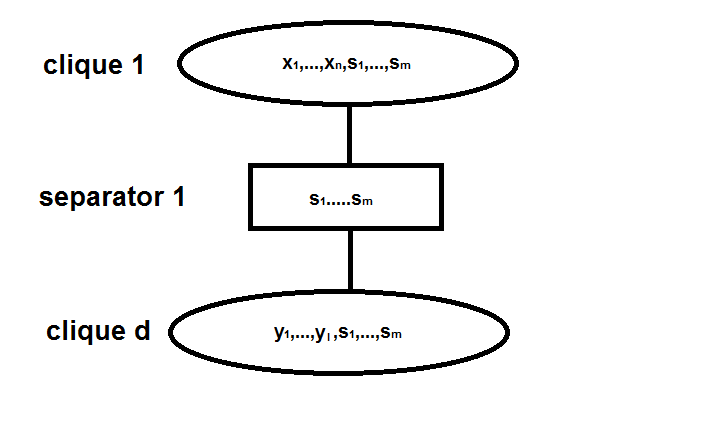
\includegraphics[width=1\textwidth]{c6e12cliques}\end{center}  
	
	In this drawing, variables $x_1,...,x_n$ are variables that exist only in clique 1 (and are the ones we sum over). Since clique 1 is a 'leaf' node of the junction tree, this means that indeed those variables exist only in this clique and once we sum over them in clique 1, they have been summed over in the entire joint distribution. Variables $s_1,...,s_m$ are the ones shared by clique 1 and clique d and once again, because clique 1 is a 'leaf' node, this means they only exist in clique 1 and clique d. Variables $y_1,...,y_l$ are the variables that exist in clique d, but not in clique 1 or separator 1. When creating a junction tree, we have to assign potentials to the cliques. In this example, there may have been potentials with variables only in $x$, such as $\phi(x_i,x_j)$. All of these would have been assigned to clique 1. There might also have been potentials with variables only in $s$, which could have been assigned either to clique 1 or clique d and there might have also been potentials with variables in both $x$ and $s$, which would have been assigned to clique 1. By summing over the variables $x$, this means that in the new "joint distribution", if we want to make a junction tree we now need to know where to assign the potentials containing variables $s$. As we said though, these variables existed only in clique 1 and clique d, therefore, all of the potentials containing variables $s$ will have to be assigned to clique d this time. More specifically suppose we had the following case where we assigned all the potentials with variables only in $s$ to clique 1:
	\begin{align*}
	clique\ 1&:\phi(X_1) = \phi(x)\phi(x,s)\phi(s)\\
	separator\ 1&:\phi(S_1) = 1\\
	clique\ d&:\phi(X_d) = \phi(y)\phi(y,s)\\
	\end{align*}
	After summing over the variables $x$, then $\phi(x,s)$ will become a new potential $\phi^n(s)$ and will be passed to clique d, just like the initial $\phi(s)$. Therefore the new clique d will consist of: $\phi^n(X_d)=\phi(y)\phi(y,s)\phi(s)\phi^n(s)$. This is also exactly what happens during the forward absorption and explains why it does not matter where we assign the potentials with variables in the separator set. Specifically, we would have:
	\begin{align*}
	&\phi(X_1) = \phi(x)\phi(x,s)\phi(s)\\
	&\phi(S_1) = 1\\
	&\phi(X_d) = \phi(y)\phi(y,s)\\
	&\phi'(S_1) = \sum_{x}\phi(X_1)=\sum_{x}\phi(x)\phi(x,s)\phi(s)\\
	&\phi'(X_d) = \phi(X_d)\frac{\phi'(S_1)}{\phi(S_1)}=\phi(X_d)\frac{\sum_{x}\phi(X_1)}{\phi(S_1)}\\
	&p(X_2,...,X_n)=\phi'(X_d)\frac{\prod_{c \geq 2,c\neq d}\phi(X_c)}{\prod_{s \geq 2}\phi(X_s)}
	\end{align*}	
	
	2. Since in the original distribution, there is no term $\frac{1}{Z}$, we can assume the global normalization constant has been "integrated" into some potential (this means that after finishing the forward elimination, the resulting potential will not need to be normalized by summing over its states). In any case, as we showed earlier, every time we sum over the variables in a clique corresponding to a leaf node, but only the variables which are not in the separator set, we are basically left with the marginal of the original distribution, but without the variables we summed over. This is all based on the fact that those variables exist only in that specific leaf node clique, otherwise this would not be possible. Therefore, it is clear that in the end we will only be left over with the variables in clique N and it will be $p(X_n)$.
	
	3. As we said earlier, at every step of the forward elimination, we are left with a junction tree which represents the marginal over all the variables that still exist in the junction tree. When we only had two cliques left over, the junction tree will represent $p(X_{n-1},X_n)$, which, if we assume the same symbolism as in part 1, where $x$ are the variables existing only in clique n, $s$ are the variables which exist in both clique n and n-1 and $y$ are the variables existing only in clique n-1, then we have $p(X_{n-1},X_n)=p(x,s,y)$. By now reversing the elimination schedule, we are summing over the variables $x$ and therefore we will be left over with the variables $s,y$ which are the variables in $X_{n-1}$ and therefore the clique will now represent the marginal $p(X_{n-1})$. Going another step back when we had still 3 cliques left over, they represented $p(X_n,X_{n-1},X_{n-2})$. We have already summed over the variables $x$, so we are left with $p(X_{n-1},X_{n-2})$. By repeating the process, we are left with $p(X_{n-2})$. Continuing, we can see how we are left with the marginals in every clique.
	
	4. By globally consistent, we mean that if cliques $X_i$ and $X_j$ share the variable $x_k$, then this must be true: $\sum_{X_i \SLASH x_k} \phi''(X_i) = \sum_{X_j \SLASH x_k} \phi''(X_j)$. However this is indeed true, since now $\phi''(X_i)=p(X_i),\phi''(X_j)=p(X_j)$, which means: $\sum_{X_i \SLASH x_k} p(X_i) = \sum_{X_j \SLASH x_k} p(X_j) \rightarrow p(x_k)=p(x_k)$. 


\end{document}





















